\documentclass[tikz,border=10pt]{standalone}
\usepackage{lmodern}        % Latin Modern fonts - prevents font warnings
\usepackage[T1]{fontenc}    % Proper font encoding
\usepackage{tikz}
\usepackage{xcolor}
\usetikzlibrary{shapes.geometric,arrows.meta,positioning,fit,patterns,calc}

% Color definitions
\definecolor{userspace}{RGB}{173,216,230}
\definecolor{kernelspace}{RGB}{255,165,79}
\definecolor{cpuhw}{RGB}{169,169,169}
\definecolor{transition}{RGB}{220,20,60}
\definecolor{datastructure}{RGB}{144,238,144}

\begin{document}
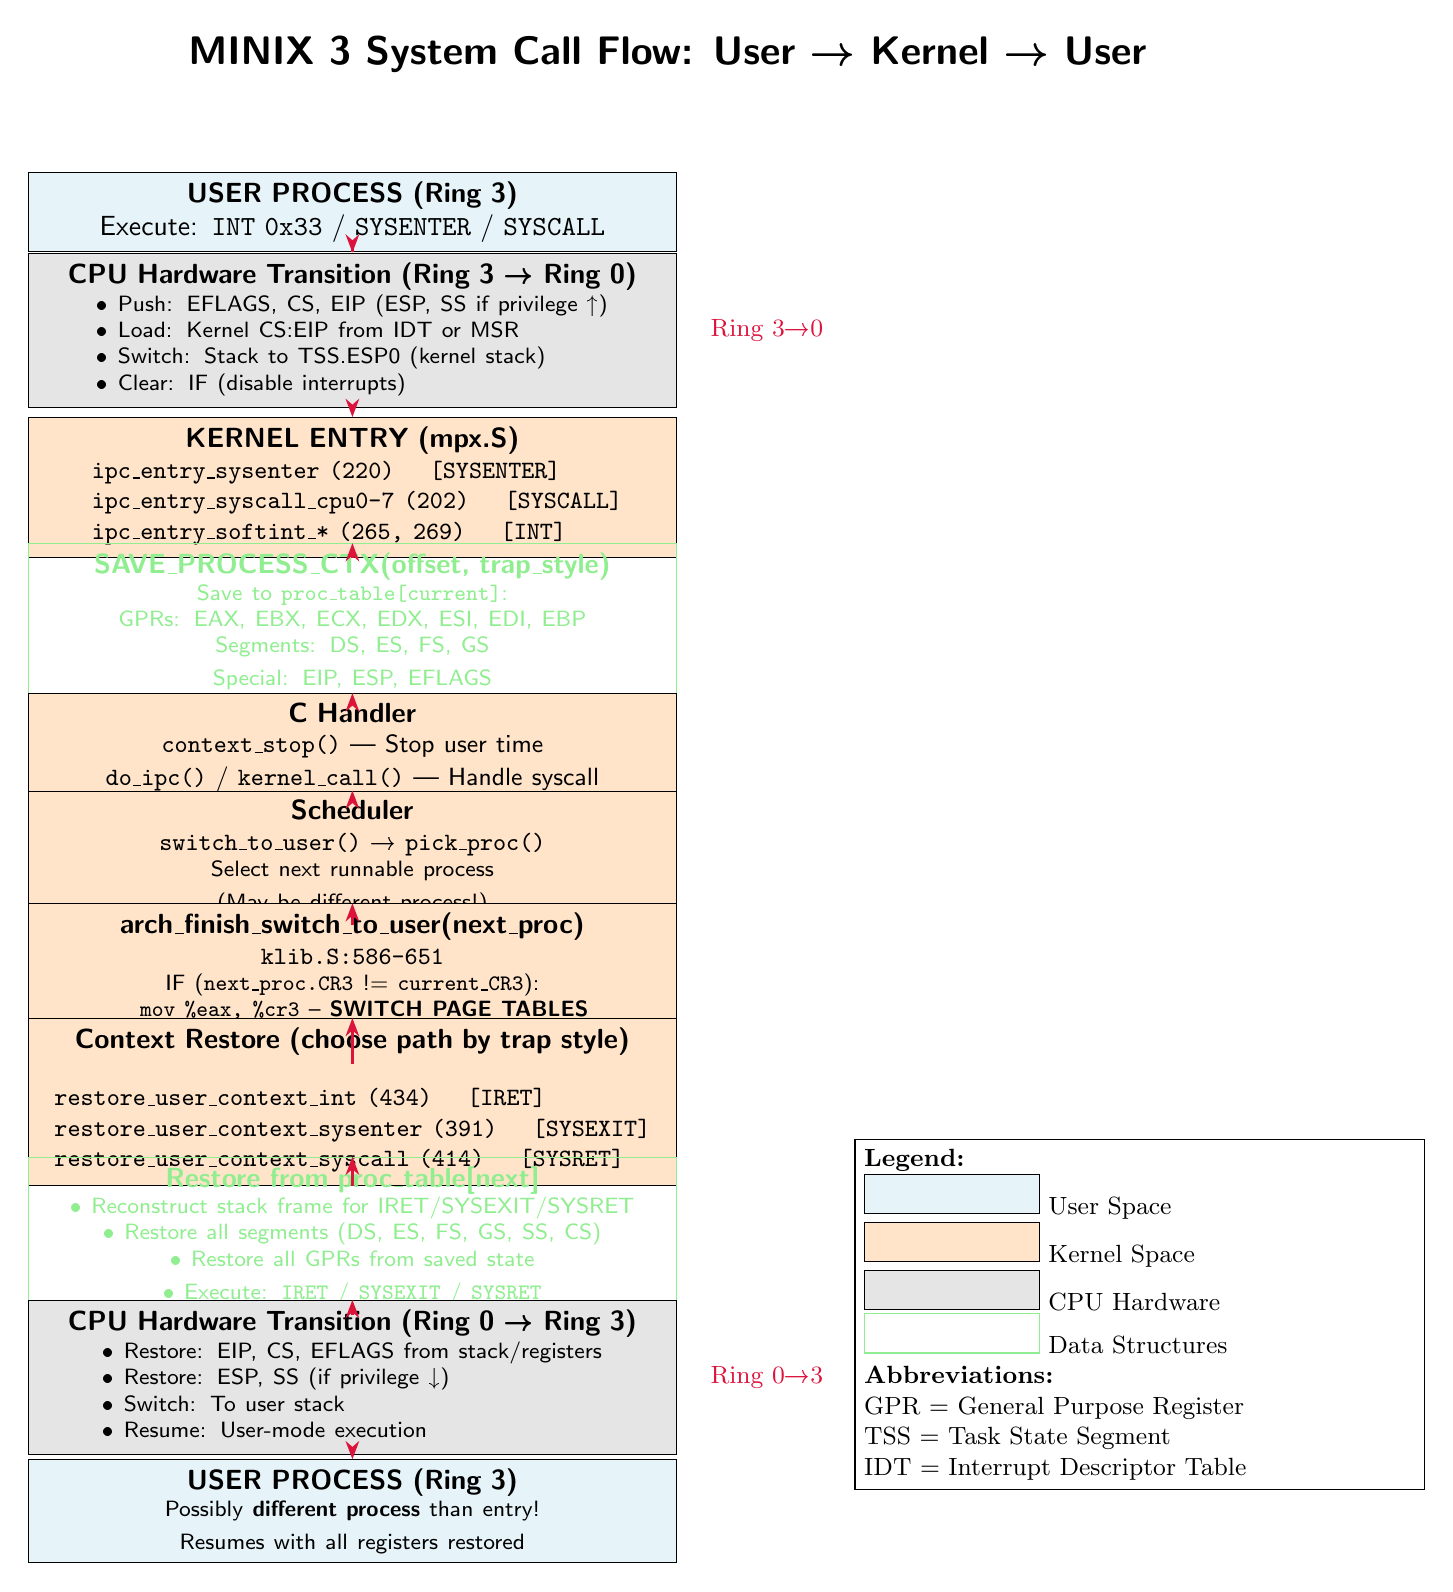
\begin{tikzpicture}[
    node distance=0.8cm,
    every node/.style={font=\sffamily},
    box/.style={rectangle, draw, text width=8cm, align=center, minimum height=1cm},
    userbox/.style={box, fill=userspace!30},
    kernelbox/.style={box, fill=kernelspace!30},
    cpubox/.style={box, fill=cpuhw!30},
    arrow/.style={-Stealth, thick, color=transition},
    label/.style={font=\ttfamily\small},
]

% Title
\node[font=\sffamily\Large\bfseries] at (4, 13) {MINIX 3 System Call Flow: User → Kernel → User};

% User space (top)
\node[userbox] (user1) at (0,11) {\textbf{USER PROCESS (Ring 3)}\\Execute: \texttt{INT 0x33} / \texttt{SYSENTER} / \texttt{SYSCALL}};

% CPU transition down
\node[cpubox] (cpu_down) at (0,9.5) {
    \textbf{CPU Hardware Transition (Ring 3 → Ring 0)}\\
    \footnotesize
    \begin{tabular}{l}
    • Push: EFLAGS, CS, EIP (ESP, SS if privilege ↑) \\
    • Load: Kernel CS:EIP from IDT or MSR \\
    • Switch: Stack to TSS.ESP0 (kernel stack) \\
    • Clear: IF (disable interrupts)
    \end{tabular}
};

% Kernel entry
\node[kernelbox] (entry) at (0,7.5) {
    \textbf{KERNEL ENTRY (mpx.S)}\\
    \small\texttt{
    \begin{tabular}{l}
    ipc\_entry\_sysenter (220) \quad [SYSENTER] \\
    ipc\_entry\_syscall\_cpu0-7 (202) \quad [SYSCALL] \\
    ipc\_entry\_softint\_* (265, 269) \quad [INT]
    \end{tabular}
    }
};

% Context save
\node[datastructure, box] (save) at (0,5.8) {
    \textbf{SAVE\_PROCESS\_CTX(offset, trap\_style)}\\
    \footnotesize Save to \texttt{proc\_table[current]}:\\
    GPRs: EAX, EBX, ECX, EDX, ESI, EDI, EBP\\
    Segments: DS, ES, FS, GS\\
    Special: EIP, ESP, EFLAGS
};

% C handler
\node[kernelbox] (handler) at (0,4.2) {
    \textbf{C Handler}\\
    \small
    \texttt{context\_stop()} — Stop user time\\
    \texttt{do\_ipc()} / \texttt{kernel\_call()} — Handle syscall
};

% Scheduler
\node[kernelbox] (scheduler) at (0,2.8) {
    \textbf{Scheduler}\\
    \small
    \texttt{switch\_to\_user()} → \texttt{pick\_proc()}\\
    \footnotesize Select next runnable process\\
    (May be different process!)
};

% Context switch
\node[kernelbox] (switch) at (0,1.2) {
    \textbf{arch\_finish\_switch\_to\_user(next\_proc)}\\
    \small\texttt{klib.S:586-651}\\
    \footnotesize
    IF (\texttt{next\_proc.CR3} != \texttt{current\_CR3}):\\
    \quad \texttt{mov \%eax, \%cr3} -- \textbf{SWITCH PAGE TABLES}\\
    Update \texttt{TSS.ESP0}
};

% Arrows down
\draw[arrow] (user1) -- (cpu_down);
\draw[arrow] (cpu_down) -- (entry);
\draw[arrow] (entry) -- (save);
\draw[arrow] (save) -- (handler);
\draw[arrow] (handler) -- (scheduler);
\draw[arrow] (scheduler) -- (switch);

% --- RETURN PATH ---
\node[kernelbox] (restore) at (0,-0.3) {
    \textbf{Context Restore (choose path by trap style)}\\
    \small\texttt{
    \begin{tabular}{l}
    restore\_user\_context\_int (434) \quad [IRET] \\
    restore\_user\_context\_sysenter (391) \quad [SYSEXIT] \\
    restore\_user\_context\_syscall (414) \quad [SYSRET]
    \end{tabular}
    }
};

\node[datastructure, box] (load) at (0,-2.0) {
    \textbf{Restore from proc\_table[next]}\\
    \footnotesize
    • Reconstruct stack frame for IRET/SYSEXIT/SYSRET\\
    • Restore all segments (DS, ES, FS, GS, SS, CS)\\
    • Restore all GPRs from saved state\\
    • Execute: \texttt{IRET} / \texttt{SYSEXIT} / \texttt{SYSRET}
};

\node[cpubox] (cpu_up) at (0,-3.8) {
    \textbf{CPU Hardware Transition (Ring 0 → Ring 3)}\\
    \footnotesize
    \begin{tabular}{l}
    • Restore: EIP, CS, EFLAGS from stack/registers \\
    • Restore: ESP, SS (if privilege ↓) \\
    • Switch: To user stack \\
    • Resume: User-mode execution
    \end{tabular}
};

\node[userbox] (user2) at (0,-5.5) {
    \textbf{USER PROCESS (Ring 3)}\\
    \footnotesize Possibly \textbf{different process} than entry!\\
    Resumes with all registers restored
};

% Arrows up
\draw[arrow] (switch) -- (restore);
\draw[arrow] (restore) -- (load);
\draw[arrow] (load) -- (cpu_up);
\draw[arrow] (cpu_up) -- (user2);

% Side annotations
\node[font=\small, text=transition, right=0.3cm of cpu_down] (ann1) {Ring 3→0};
\node[font=\small, text=transition, right=0.3cm of cpu_up] (ann2) {Ring 0→3};

% Legend
\node[draw, fill=white, font=\small, text width=7cm] at (10, -3) {
    \textbf{Legend:}\\
    \tikz\node[userbox,minimum height=0.5cm,text width=2cm]{};  User Space\\
    \tikz\node[kernelbox,minimum height=0.5cm,text width=2cm]{}; Kernel Space\\
    \tikz\node[cpubox,minimum height=0.5cm,text width=2cm]{}; CPU Hardware\\
    \tikz\node[datastructure,box,minimum height=0.5cm,text width=2cm]{}; Data Structures

    \textbf{Abbreviations:}\\
    GPR = General Purpose Register\\
    TSS = Task State Segment\\
    IDT = Interrupt Descriptor Table
};

\end{tikzpicture}
\end{document}
